
%%% main document {{{

\documentclass[
a4paper,     %% defines the paper size: a4paper (default), a5paper, letterpaper, ...
% landscape,   %% sets the orientation to landscape
% twoside,     %% changes to a two-page-layout (alternatively: oneside)
% twocolumn,   %% changes to a two-column-layout
 headsepline, %% add a horizontal line below the column title
% footsepline, %% add a horizontal line above the page footer
% titlepage,   %% only the titlepage (using titlepage-environment) appears on the first page (alternatively: notitlepage)
% parskip,     %% insert an empty line between two paragraphs (alternatively: halfparskip, ...)
% leqno,       %% equation numbers left (instead of right)
% fleqn,       %% equation left-justified (instead of centered)
% tablecaptionabove, %% captions of tables are above the tables (alternatively: tablecaptionbelow)
% draft,       %% produce only a draft version (mark lines that need manual edition and don't show graphics)
% 10pt         %% set default font size to 10 point
11pt         %% set default font size to 11 point
% 12pt         %% set default font size to 12 point
]{scrartcl}  %% article, see KOMA documentation (scrguide.dvi)



%%%%%%%%%%%%%%%%%%%%%%%%%%%%%%%%%%%%%%%%%%%%%%%%%%%%%%%%%%%%%%%%%%%%%%%%%%%%%%%%
%%%
%%% packages
%%%

%%%
%%% encoding and language set
%%%

%%% ngerman: language set to new-german
\usepackage{ngerman}

%%% babel: language set (can cause some conflicts with package ngerman)
%%%        use it only for multi-language documents or non-german ones
%\usepackage[ngerman]{babel}

%%% inputenc: coding of german special characters
\usepackage[utf8]{inputenc}

%%% fontenc, ae, aecompl: coding of characters in PDF documents
\usepackage[T1]{fontenc}
\usepackage{ae,aecompl}

%%%
%%% technical packages
%%%

%%% amsmath, amssymb, amstext: support for mathematics
%\usepackage{amsmath,amssymb,amstext}

%%% psfrag: replace PostScript fonts
\usepackage{psfrag}

%%% listings: include programming code
%\usepackage{listings}

%%% units: technical units
\usepackage{units}

%%% tiefgestellte zahlen
\usepackage{subscript}

%%% mathefoo
\usepackage{amsmath}


\usepackage{xcolor}
% TikZ-Bibliotheken
\usepackage{tikz}
 \usetikzlibrary{backgrounds}
 \usetikzlibrary{matrix}
 \usetikzlibrary{circuits.ee.IEC}
 \usetikzlibrary{positioning}
 
 
%Hintergrundstyle - optional
\tikzstyle{background rectangle}=
  [thick,draw=\lightgray, fill=white!99!black, rounded corners]
 
%Volt- und Amperemeter festlegen:
\tikzset{circuit declare symbol = ammeter}
\tikzset{set ammeter graphic ={draw,generic circle IEC, minimum size=5mm,info=center:A}}
\tikzset{circuit declare symbol = voltmeter}
\tikzset{set voltmeter graphic ={draw,generic circle IEC, minimum size=5mm,info=center:V}}
\tikzset{circuit declare symbol = generator}
\tikzset{set generator graphic ={draw,rectangle ee, minimum size=5mm,info=center:G}}
% Spannungs und Strompfeile
\tikzset{
  Pfeil/.style={thick,shorten >=#1,shorten <=#1,->}, % für Peile
  UPfeil/.style={blue,Pfeil=#1,font={\sffamily\itshape}},% für Spannungspfeile
  IPfeil/.style={red,Pfeil=#1,font={\ttfamily\itshape}} % für Strompfeile
}


%Boxen
\usepackage{empheq}
 
% Command "alignedbox{}{}" for a box within an align environment
% Source: http://www.latex-community.org/forum/viewtopic.php?f=46&t=8144
\newlength\dlf  % Define a new measure, dlf
\newcommand\alignedbox[2]{
% Argument #1 = before & if there were no box (lhs)
% Argument #2 = after & if there were no box (rhs)
&  % Alignment sign of the line
{
\settowidth\dlf{$\displaystyle #1$}  
    % The width of \dlf is the width of the lhs, with a displaystyle font
\addtolength\dlf{\fboxsep+\fboxrule}  
    % Add to it the distance to the box, and the width of the line of the box
\hspace{-\dlf}  
    % Move everything dlf units to the left, so that & #1 #2 is aligned under #1 & #2
\boxed{#1 #2}
    % Put a box around lhs and rhs
}
}

%%%
%%% layout
%%%

%%% scrpage2: KOMA heading and footer
%%% Note: if you don't use this package, please remove 
%%%       \pagestyle{scrheadings} and corresponding settings
%%%       below too.
\usepackage[automark]{scrpage2}


%%%
%%% PDF
%%%

\usepackage{ifpdf}

%%% Should be LAST usepackage-call!
%%% For docu on that, see reference on package ``hyperref''
\ifpdf%   (definitions for using pdflatex instead of latex)

  %%% graphicx: support for graphics
  %\usepackage[pdftex]{graphicx}

  \pdfcompresslevel=9

  %%% hyperref (hyperlinks in PDF): for more options or more detailed
  %%%          explanations, see the documentation of the hyperref-package
  \usepackage[%
    %%% general options
    pdftex=true,      %% sets up hyperref for use with the pdftex program
    %plainpages=false, %% set it to false, if pdflatex complains: ``destination with same identifier already exists''
    %
    %%% extension options
    backref,      %% adds a backlink text to the end of each item in the bibliography
    pagebackref=false, %% if true, creates backward references as a list of page numbers in the bibliography
    colorlinks=true,   %% turn on colored links (true is better for on-screen reading, false is better for printout versions)
    %
    %%% PDF-specific display options
    bookmarks=true,          %% if true, generate PDF bookmarks (requires two passes of pdflatex)
    bookmarksopen=false,     %% if true, show all PDF bookmarks expanded
    bookmarksnumbered=false, %% if true, add the section numbers to the bookmarks
    %pdfstartpage={1},        %% determines, on which page the PDF file is opened
    pdfpagemode=None         %% None, UseOutlines (=show bookmarks), UseThumbs (show thumbnails), FullScreen
  ]{hyperref}


  %%% provide all graphics (also) in this format, so you don't have
  %%% to add the file extensions to the \includegraphics-command
  %%% and/or you don't have to distinguish between generating
  %%% dvi/ps (through latex) and pdf (through pdflatex)
  \DeclareGraphicsExtensions{.pdf}

\else %else   (definitions for using latex instead of pdflatex)

  \usepackage[dvips]{graphicx}

  \DeclareGraphicsExtensions{.eps}

  \usepackage[%
    dvips,           %% sets up hyperref for use with the dvips driver
    colorlinks=false %% better for printout version; almost every hyperref-extension is eliminated by using dvips
  ]{hyperref}

\fi


%%% sets the PDF-Information options
%%% (see fields in Acrobat Reader: ``File -> Document properties -> Summary'')
%%% Note: this method is better than as options of the hyperref-package (options are expanded correctly)
\hypersetup{
  pdftitle={}, %%
  pdfauthor={}, %%
  pdfsubject={}, %%
  pdfcreator={Accomplished with LaTeX2e and pdfLaTeX with hyperref-package.}, %% 
  pdfproducer={}, %%
  pdfkeywords={} %%
}


%%%%%%%%%%%%%%%%%%%%%%%%%%%%%%%%%%%%%%%%%%%%%%%%%%%%%%%%%%%%%%%%%%%%%%%%%%%%%%%%
%%%
%%% user defined commands
%%%

%%% \mygraphics{}{}{}
%% usage:   \mygraphics{width}{filename_without_extension}{caption}
%% example: \mygraphics{0.7\textwidth}{rolling_grandma}{This is my grandmother on inlinescates}
%% requires: package graphicx
%% provides: including centered pictures/graphics with a boldfaced caption below
%% 
\newcommand{\mygraphics}[3]{
  \begin{center}
    \includegraphics[width=#1, keepaspectratio=true]{#2} \\
    \textbf{#3}
  \end{center}
}

%%%%%%%%%%%%%%%%%%%%%%%%%%%%%%%%%%%%%%%%%%%%%%%%%%%%%%%%%%%%%%%%%%%%%%%%%%%%%%%%
%%%
%%% define the titlepage
%%%

% \subject{}   %% subject which appears above titlehead
% \titlehead{} %% special heading for the titlepage

%%% title
\title{Messbericht Parallelschaltung}

%%% author(s)
\author{Felix Schiller \\ Sebastian Littau \\ E1FS2}

%%% date
\date{Reutlingen, am 15.12.2015}

% \publishers{}

% \thanks{} %% use it instead of footnotes (only on titlepage)

% \dedication{} %% generates a dedication-page after titlepage


%%% uncomment following lines, if you want to:
%%% reuse the maketitle-entries for hyperref-setup
%\newcommand\org@maketitle{}
%\let\org@maketitle\maketitle
%\def\maketitle{%
%  \hypersetup{
%    pdftitle={\@title},
%    pdfauthor={\@author}
%    pdfsubject={\@subject}
%  }%
%  \org@maketitle
%}


%%%%%%%%%%%%%%%%%%%%%%%%%%%%%%%%%%%%%%%%%%%%%%%%%%%%%%%%%%%%%%%%%%%%%%%%%%%%%%%%
%%%
%%% set heading and footer
%%%

%%% scrheadings default: 
%%%      footer - middle: page number
\pagestyle{scrheadings}

%%% user specific
%%% usage:
%%% \position[heading/footer for the titlepage]{heading/footer for the rest of the document}

%%% heading - left
\ihead[]{Schiller, Felix \\ Littau, Sebastian}

%%% heading - center
\chead[]{Messbericht \\Parallelschaltung}

%%% heading - right
\ohead[]{\thepage}

%%% footer - left
% \ifoot[]{}

%%% footer - center
% \cfoot[]{}

%%% footer - right
% \ofoot[]{}



%%%%%%%%%%%%%%%%%%%%%%%%%%%%%%%%%%%%%%%%%%%%%%%%%%%%%%%%%%%%%%%%%%%%%%%%%%%%%%%%
%%%
%%% begin document
%%%

\begin{document}

% \pagenumbering{roman} %% small roman page numbers

%%% include the title
% \thispagestyle{empty}  %% no header/footer (only) on this page
\maketitle

%%% start a new page and display the table of contents
\newpage
\tableofcontents

%%% start a new page and display the list of figures
% \newpage
% \listoffigures

%%% start a new page and display the list of tables
% \newpage
% \listoftables

%%% display the main document on a new page 
% \newpage

% \pagenumbering{arabic} %% normal page numbers (include it, if roman was used above)

%%%%%%%%%%%%%%%%%%%%%%%%%%%%%%%%%%%%%%%%%%%%%%%%%%%%%%%%%%%%%%%%%%%%%%%%%%%%%%%%
%%%
%%% begin main document
%%% structure: \section \subsection \subsubsection \paragraph \subparagraph
%%%
\section{Messaufgabe}
An einer Parallelschaltung von 4 Widerständen soll durch Messung ermittelt werden, wie sich 
\begin{enumerate}
	\item die Ströme zwischen den einzelnen Bauteilen und 
	\item die Spannungen an den einzelnen Bauteilen verhalten. 
\end{enumerate}
Die messtechnisch gewonnenen Ergebnisse sind so zu verallgemeinern, dass sie auf beliebige Parallelschaltungen anwendbar sind.

\section{Messung}
\subsection{Stromabhängigkeit}
\subsection{Messschaltung zur Bestimmung der Ströme zwischen den Bauteilen}

\begin{center}
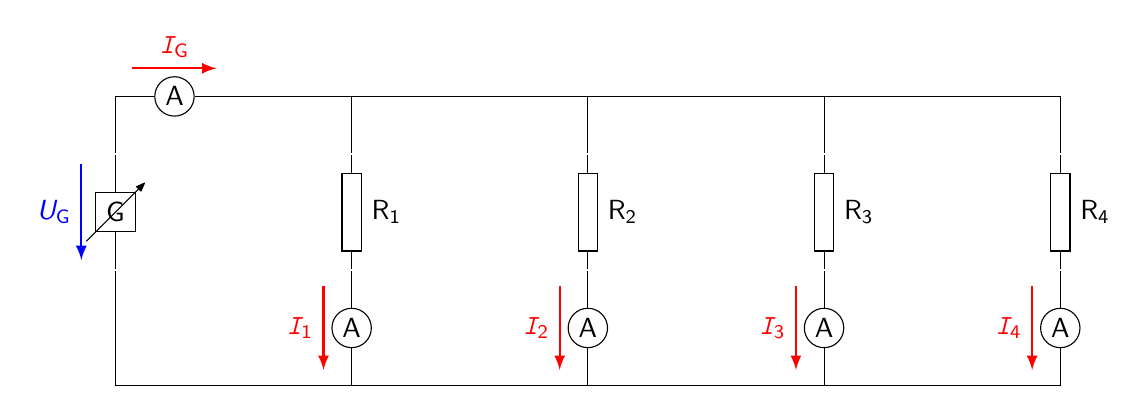
\begin{tikzpicture}[%show background rectangle,
circuit ee IEC, circuit symbol lines/.style={draw,thick},
font=\sffamily\upshape,
>=latex % Voreinstellung für Pfeilspitzen
]
\matrix (S) [
  matrix of nodes, nodes in empty cells,
  inner sep=0pt, outer sep=-.5\pgflinewidth,
  column sep=15mm, row sep = 7mm,
  nodes={minimum width=0pt}
  ]
{
  &&&&&&&&  \\
  &&&&&&&&  \\
  &&&&&&&&  \\
  &&&&&&&&  \\
  &&&&&&&&  \\
  &&&&&&&&  \\
};
 
 
%Orientierungshilfen
%\foreach \j in {1,...,6}
% \foreach \k in {1,...,9}{%
%\node[text=lightgray] at (S-\j-\k){+}; % Orientierungshilfe +
%\node[red, left] at (S-\j-1){\j}; %Orientierungshilfe Zeilennummer
%\node[red, above] at (S-1-\k){\k}; %Orientierungshilfe Spaltennummer  
%};%
 

%Bauteile
\draw (S-4-1) to  [generator={adjustable', name=Gen}](S-2-1);

\draw (S-2-3) to  [resistor={info=R$_\mathsf{1}$, name=Wstd}](S-4-3);
\draw (S-4-3) to  [ammeter ={name=AM1}](S-6-3);
%\draw (S-2-2) to  [voltmeter ={name=VM1}](S-4-2);

\draw (S-2-5) to  [resistor={info=R$_\mathsf{2}$, name=Wstd}](S-4-5);
\draw (S-4-5) to  [ammeter ={name=AM2}](S-6-5);
%\draw (S-2-4) to  [voltmeter ={name=VM2}](S-4-4);

\draw (S-2-7) to  [resistor={info=R$_\mathsf{3}$, name=Wstd}](S-4-7);
\draw (S-4-7) to  [ammeter ={name=AM3}](S-6-7);
%\draw (S-2-6) to  [voltmeter ={name=VM3}](S-4-6);

\draw (S-2-9) to  [resistor={info=R$_\mathsf{4}$, name=Wstd}](S-4-9);
\draw (S-4-9) to  [ammeter ={name=AM4}](S-6-9);
%\draw (S-2-8) to  [voltmeter ={name=VM4}](S-4-8);

\draw (S-1-1) to  [ammeter ={name=AMg}](S-1-2);

%Spannungspfeile
%Spannungspfeil der Quelle / des Voltmeters
\draw[UPfeil=-1em]([xshift=-.5em]Gen.north west) -- node [left]{U$\mathsf{_G}$}([xshift=-.5em]Gen.south west);
%\draw[UPfeil=-1em]([xshift=.5em]VM1.north east) -- node [right]{U$\mathsf{_1}$}([xshift=.5em]VM1.south east);
%\draw[UPfeil=-1em]([xshift=.5em]VM2.north east) -- node [right]{U$\mathsf{_2}$}([xshift=.5em]VM2.south east);
%\draw[UPfeil=-1em]([xshift=.5em]VM3.north east) -- node [right]{U$\mathsf{_3}$}([xshift=.5em]VM3.south east);
%\draw[UPfeil=-1em]([xshift=.5em]VM4.north east) -- node [right]{U$\mathsf{_4}$}([xshift=.5em]VM4.south east);

%Strompfeile
\draw[IPfeil=-1em]([xshift=-.5em]AM1.north west) -- node [left]{I$\mathsf{_1}$}([xshift=-.5em]AM1.south west);
\draw[IPfeil=-1em]([xshift=-.5em]AM2.north west) -- node [left]{I$\mathsf{_2}$}([xshift=-.5em]AM2.south west); 
\draw[IPfeil=-1em]([xshift=-.5em]AM3.north west) -- node [left]{I$\mathsf{_3}$}([xshift=-.5em]AM3.south west); 
\draw[IPfeil=-1em]([xshift=-.5em]AM4.north west) -- node [left]{I$\mathsf{_4}$}([xshift=-.5em]AM4.south west);
\draw[IPfeil=-1em]([yshift=.5em]AMg.north west) -- node [above]{I$\mathsf{_G}$}([yshift=.5em]AMg.north east);
 
%Leiterbahnen
\draw (S-1-1) -- (S-2-1);
\draw (S-1-2) -- (S-1-9);

\draw (S-1-3) -- (S-2-3);
\draw (S-1-5) -- (S-2-5);
\draw (S-1-7) -- (S-2-7);
\draw (S-1-9) -- (S-2-9);

%\draw (S-2-2) -- (S-2-3);
%\draw (S-2-4) -- (S-2-5);
%\draw (S-2-6) -- (S-2-7);
%\draw (S-2-8) -- (S-2-9);

%\draw (S-4-2) -- (S-4-3);
%\draw (S-4-4) -- (S-4-5);
%\draw (S-4-6) -- (S-4-7);
%\draw (S-4-8) -- (S-4-9);

\draw (S-6-1) -- (S-6-9);
\draw (S-4-1) -- (S-6-1);
 
 
\end{tikzpicture}
\end{center}

\subsection{Aufbau der Schaltung}

In der oben skizzierten Schaltung sind die Widerstände $R_{1..4}$ parallel an die Spannungsquelle angeschlossen. 
Die Widerstandswerte betragen $ R_1 = 150 \Omega, R_2 = 220 \Omega, R_3=470 \Omega, R_4=820 \Omega$. 
Als Speisespannung wird $ U_G = 10V$ angelegt. 
Mit den Messgeräten, die mit den Widerständen in Reihe geschaltet sind können die Ströme $I_{1..4}$ in den einzelnen Widerständen, sowie der Gesamtstrom $I_G$ durch die Schaltung gemessen werden.

\subsection{Messwerte und Zusammenhänge}

In der oben beschrieben Schaltung wurden die folgenden Ströme gemessen:
\begin{center}
  \begin{tabular}{ l | c | c | c | c | c}
    \hline
    Strom      & I\textsubscript{G} & I\textsubscript{1} & I\textsubscript{2} & I\textsubscript{3} & I\textsubscript{4}  \\ \hline
    Wert in mA & 145 & 67 & 45 & 21,5 & 12 \\
    \hline
  \end{tabular}
\end{center}
Der Gesamtstrom, der durch die Schaltung fließt teilt sich entsprechend der Werte der einzelenn Widerstände auf.
\begin{align}
I_G &= I_1 + I_2 + I_3 + I_4 \nonumber \\
    &= 67mA + 45mA + 21,5mA + 12mA \nonumber \\
    &= 145,5 mA \nonumber
\end{align}
Der Strom $I_G$ enspricht der Summe der einzelnen Ströme $I_{1..4}$.\newline
Die Abweichung zwischen dem gemessenen und dem errechneten Gesamtstrom ergibt sich aus den verschiedenen Ungenauigkeiten. 
Die verschiedenen Messbereiche des verwendeten Unigor A43 haben verschiedene Innenwiderstände, die sich auf die gemessenen Werte auswirken. 
Dazu kommen noch Ablesefehler auf der analogen Messskala.

\subsection{Spannungsabhängigkeit}
\subsection{Messschaltung zur Messung der Spannung über die einzelnen Bauteile}

\begin{center}
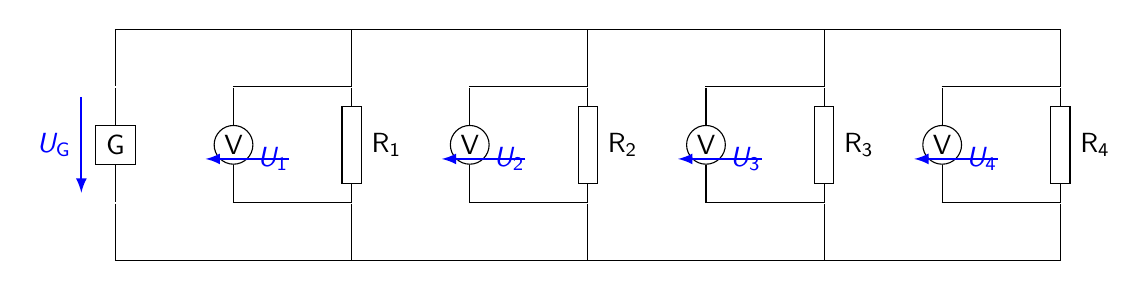
\begin{tikzpicture}[%show background rectangle,
circuit ee IEC, circuit symbol lines/.style={draw,thick},
font=\sffamily\upshape,
>=latex % Voreinstellung für Pfeilspitzen
]
\matrix (S) [
  matrix of nodes, nodes in empty cells,
  inner sep=0pt, outer sep=-.5\pgflinewidth,
  column sep=15mm, row sep = 7mm,
  nodes={minimum width=0pt}
  ]
{
  &&&&&&&&  \\
  &&&&&&&&  \\
  &&&&&&&&  \\
  &&&&&&&&  \\
  &&&&&&&&  \\
};
 
 
%Orientierungshilfen
%\foreach \j in {1,...,5}
% \foreach \k in {1,...,9}{%
%\node[text=lightgray] at (S-\j-\k){+}; % Orientierungshilfe +
%\node[red, left] at (S-\j-1){\j}; %Orientierungshilfe Zeilennummer
%\node[red, above] at (S-1-\k){\k}; %Orientierungshilfe Spaltennummer  
%};%
 

%Bauteile
\draw (S-4-1) to  [generator={name=Gen}](S-2-1);

\draw (S-2-3) to  [resistor={info=R$_\mathsf{1}$, name=Wstd}](S-4-3);
%\draw (S-4-3) to  [ammeter ={name=AM1}](S-6-3);
\draw (S-2-2) to  [voltmeter ={name=VM1}](S-4-2);

\draw (S-2-5) to  [resistor={info=R$_\mathsf{2}$, name=Wstd}](S-4-5);
%\draw (S-4-5) to  [ammeter ={name=AM2}](S-6-5);
\draw (S-2-4) to  [voltmeter ={name=VM2}](S-4-4);

\draw (S-2-7) to  [resistor={info=R$_\mathsf{3}$, name=Wstd}](S-4-7);
%\draw (S-4-7) to  [ammeter ={name=AM3}](S-6-7);
\draw (S-2-6) to  [voltmeter ={name=VM3}](S-4-6);

\draw (S-2-9) to  [resistor={info=R$_\mathsf{4}$, name=Wstd}](S-4-9);
%\draw (S-4-9) to  [ammeter ={name=AM4}](S-6-9);
\draw (S-2-8) to  [voltmeter ={name=VM4}](S-4-8);

%\draw (S-1-1) to  [ammeter ={name=AMg}](S-1-2);

%Spannungspfeile
%Spannungspfeil der Quelle / des Voltmeters
\draw[UPfeil=-1em]([xshift=-.5em]Gen.north west) -- node [left]{U$\mathsf{_G}$}([xshift=-.5em]Gen.south west);
\draw[UPfeil=-1em]([xshift=.5em]VM1.north east) -- node [right]{U$\mathsf{_1}$}([xshift=.5em]VM1.south east);
\draw[UPfeil=-1em]([xshift=.5em]VM2.north east) -- node [right]{U$\mathsf{_2}$}([xshift=.5em]VM2.south east);
\draw[UPfeil=-1em]([xshift=.5em]VM3.north east) -- node [right]{U$\mathsf{_3}$}([xshift=.5em]VM3.south east);
\draw[UPfeil=-1em]([xshift=.5em]VM4.north east) -- node [right]{U$\mathsf{_4}$}([xshift=.5em]VM4.south east);

%Strompfeile
%\draw[IPfeil=-1em]([xshift=-.5em]AM1.north west) -- node [left]{I$\mathsf{_1}$}([xshift=-.5em]AM1.south west);
%\draw[IPfeil=-1em]([xshift=-.5em]AM2.north west) -- node [left]{I$\mathsf{_2}$}([xshift=-.5em]AM2.south west); 
%\draw[IPfeil=-1em]([xshift=-.5em]AM3.north west) -- node [left]{I$\mathsf{_3}$}([xshift=-.5em]AM3.south west); 
%\draw[IPfeil=-1em]([xshift=-.5em]AM4.north west) -- node [left]{I$\mathsf{_4}$}([xshift=-.5em]AM4.south west);
%\draw[IPfeil=-1em]([yshift=.5em]AMg.north west) -- node [above]{I$\mathsf{_G}$}([yshift=.5em]AMg.north east);
 
%Leiterbahnen
\draw (S-1-1) -- (S-2-1);
\draw (S-1-1) -- (S-1-9);

\draw (S-1-3) -- (S-2-3);
\draw (S-1-5) -- (S-2-5);
\draw (S-1-7) -- (S-2-7);
\draw (S-1-9) -- (S-2-9);

\draw (S-4-3) -- (S-5-3);
\draw (S-4-5) -- (S-5-5);
\draw (S-4-7) -- (S-5-7);
\draw (S-4-9) -- (S-5-9);

\draw (S-2-2) -- (S-2-3);
\draw (S-2-4) -- (S-2-5);
\draw (S-2-6) -- (S-2-7);
\draw (S-2-8) -- (S-2-9);

\draw (S-4-2) -- (S-4-3);
\draw (S-4-4) -- (S-4-5);
\draw (S-4-6) -- (S-4-7);
\draw (S-4-8) -- (S-4-9);

\draw (S-5-1) -- (S-5-9);
\draw (S-4-1) -- (S-5-1);
 
 
\end{tikzpicture}
\end{center}

\subsection{Aufbau der Schaltung}

In der oben skizzierten Schaltung sind die Widerstände $R_{1..4}$ parallel an die Spannungsquelle angeschlossen. 
Die Widerstandswerte betragen $ R_1 = 150 \Omega, R_2 = 220 \Omega, R_3=470 \Omega, R_4=820 \Omega$. 
Als Speisespannung wird $ U_G = 10V$ angelegt. 
Mit den parallel zu den Widerständen angeschlossenen Messgeräten können die Spannungen $U_{1..4}$ an den einzelnen Widerständen gemessen werden.

\subsection{Messwerte und Zusammenhänge}
In der oben beschrieben Schaltung wurden die folgenden Spannungen gemessen:
\begin{center}
  \begin{tabular}{ l | c | c | c | c | c}
    \hline
    Spannung   & U\textsubscript{G} & U\textsubscript{1} & U\textsubscript{2} & U\textsubscript{3} & U\textsubscript{4}  \\ \hline
    Wert in V  & 10,04 & 9,99 & 10,01 & 10,0 & 9,99 \\
    \hline
  \end{tabular}
\end{center}
An allen Widerständen liegt, bis auf Messfehler genau, die selbe Spannung an.
\[U_G=U_1=U_2=U_3=U_4\]


\section{Erkenntnisse}

\subsection{Wie verhalten sich die Ströme bei einer Parallelschaltung?}
Der Gesamtstrom teilt sich auf alle Widerstände auf. Durch jeden Widerstand fließt der Strom $I_n=\frac{U_G}{R_n}$.
Durch alle Widerstände zusammen fließt ein Gesamtstrom der der Summe aller Einzelströme entspricht.
\[I_G = I_1 + I_2 + I_3 + I_4\]

\subsection{Beziehung zwischen der Generatorspannung und den gemessenen Spannungen}
An jedem Widerstand liegt die selbe Spannung an. Die positive Seite eines jeden Widerstands liegt auf dem selben Potential.
\[U_G=U_1=U_2=U_3=U_4\]

\subsection{Gesamtwiderstand und Beziehung der einzelnen Widerstandswerte zum Gesamtwiderstand}
Der Gesamtwiderstand der Schaltung lässt sich aus dem gemessenen Gesamtstrom und der angelegten Spannung berechnen.
\[R_{ges} = \frac{U_G}{I_G} = \frac{10,04V}{145mA}= 69,2\Omega\]

\subsection{Mathematische Herleitung}
Aus dem Ohmschen Gesetz kann man den Gesamtwiderstand auch über den fließenden Strom herleiten.
\begin{align}
I_{G} & = I_1+I_2+I_3+I_4 \nonumber \\
\frac{U_G}{R_{ges}} &= \frac{U_1}{R_1} + \frac{U_2}{R_2} + \frac{U_3}{R_3} + \frac{U_4}{R_4} \nonumber \\
\frac{1}{R_{ges}} &= \frac{1}{R_1} + \frac{1}{R_2} + \frac{1}{R_3} + \frac{1}{R_4} \nonumber \\
\frac{1}{R_{ges}} &= \frac{1}{150\Omega} + \frac{1}{220\Omega} + \frac{1}{470\Omega} + \frac{1}{820\Omega} \nonumber \\
				  &= 0,0145 \frac{1}{\Omega} \nonumber\\
\Rightarrow R_{ges} &= 69,44\Omega \nonumber
\end{align}
Da die an allen Widerständen anliegende Spannung gleich ist kann die gesamte Gleichung durch $U_G$ geteilt werden. Dadurch wird die Spannung aus der  Gleichung eliminiert.
Mit eingesetzten Zahlen kommt man wieder auf den $ R_{ges}$, der schon oben ausgerechnet wurde.
\newpage
Eine Berechnung über Kehrwerte ist oft sehr aufwendig. Deshalb wurde eine neue Größe eingeführt, der Leitwert $G$. Er wird in Siemens angegeben und entspricht dem Kehrwert des Widerstandes.
\begin{align}
\frac{1}{R_{ges}} &= \frac{1}{R_1} + \frac{1}{R_2} + \frac{1}{R_3} + \frac{1}{R_4} \nonumber \\
\frac{1}{\frac{U_G}{I_G}} &= \frac{1}{\frac{U_1}{I_1}} + \frac{1}{\frac{U_2}{I_2}} + \frac{1}{\frac{U_3}{I_3}} + \frac{1}{\frac{U_4}{I_4}} \nonumber \\
\frac{I_G}{U_G} &= \frac{I_1}{U_1} + \frac{I_2}{U_2} + \frac{I_3}{U_3} + \frac{I_4}{U_4} \nonumber \\
G_{ges} &= G_1 + G_2 + G_3 + G_4 \nonumber 
\end{align}
Für zwei parallel geschaltete Widerstände, ein Fall, den man in vielen Schaltungen findet lässt sich eine vereinfachte Sonderformel finden.
\begin{align}
\frac{1}{R_{ges}} &= \frac{1}{R_1} + \frac{1}{R_2} \nonumber \\
\frac{1}{R_{ges}} &= \frac{R_2}{R_1 \cdot (R_1 \cdot R_2)} + \frac{R_1}{R_2\cdot (R_1 \cdot R_2)} \nonumber \\
\frac{1}{R_{ges}} &= \frac{R_2}{R_1 \cdot R_2} + \frac{R_1}{R_1 \cdot R_2} \nonumber \\
\frac{1}{R_{ges}} &= \frac{R_2+R_1}{R_1 \cdot R_2} \nonumber \\
\alignedbox{R_{ges} }{= \frac{R_2 \cdot R_1}{R_1 + R_2}} \nonumber 
\end{align}


\section{Anwenderschaltung}
Zwei Lampen, $H_1 (12V/240mA)$ und $H_2 (12V/96mA)$ sollen an einer Spannungsquelle mit $U_G=24V$ angeschlossen werden können. Ein zusätzlicher Widerstand ist nötig beide Lampen zusammen betreiben zu können. Dieser wird parallel zu $H_2$ gesteckt.

\subsection{Schaltung}

\begin{center}
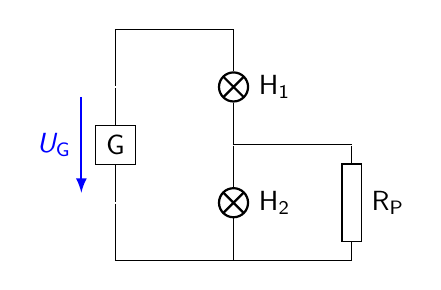
\begin{tikzpicture}[%show background rectangle,
circuit ee IEC, circuit symbol lines/.style={draw,thick},
font=\sffamily\upshape,
>=latex % Voreinstellung für Pfeilspitzen
]
\matrix (S) [
  matrix of nodes, nodes in empty cells,
  inner sep=0pt, outer sep=-.5\pgflinewidth,
  column sep=15mm, row sep = 7mm,
  nodes={minimum width=0pt}
  ]
{
  &&  \\
  &&  \\
  &&  \\
  &&  \\
  &&  \\
};
 
 
%Orientierungshilfen
%\foreach \j in {1,...,5}
% \foreach \k in {1,...,3}{%
%\node[text=lightgray] at (S-\j-\k){+}; % Orientierungshilfe +
%\node[red, left] at (S-\j-1){\j}; %Orientierungshilfe Zeilennummer
%\node[red, above] at (S-1-\k){\k}; %Orientierungshilfe Spaltennummer  
%};%
 

%Bauteile
\draw (S-4-1) to  [generator={name=Gen}](S-2-1);
\draw (S-1-2) to  [bulb={info=H$_\mathsf{1}$, name=H1}](S-3-2);
\draw (S-3-2) to  [bulb={info=H$_\mathsf{2}$, name=H2}](S-5-2);
\draw (S-3-3) to  [resistor={info=R$_\mathsf{P}$, name=Wstd}](S-5-3);


%Spannungspfeile
%Spannungspfeil der Quelle / des Voltmeters
\draw[UPfeil=-1em]([xshift=-.5em]Gen.north west) -- node [left]{U$\mathsf{_G}$}([xshift=-.5em]Gen.south west);

 
%Leiterbahnen
\draw (S-1-1) -- (S-2-1);
\draw (S-1-1) -- (S-1-2);
\draw (S-4-1) -- (S-5-1);
\draw (S-5-1) -- (S-5-3); 
\draw (S-3-2) -- (S-3-3);

\end{tikzpicture}
\end{center}

\subsection{Berechnung des Parallelwiderstands}
Die Lampe $H_1$ ist in Reihe zu der Kombination aus Lampe $H_2$ und Parallelwiderstand $R_P$. An beiden Schaltungsteilen fällt je $\frac{U_G}{2}=12V$ ab. Durch $H_2$ darf maximal ein Strom von $96mA$ fließen, der Rest muss durch den Parallelwiderstand.
\begin{align}
I_G &= I_{H_2} + I_{R_P} \nonumber \\
I_{R_P} &= I_G - I_{H_2}  \nonumber \\
I_{R_P} &= 240mA - 96mA = 144mA \nonumber
\end{align}
Also ist ein Widerstand gesucht, der bei $12V$ angelegter Spannung $144mA$ Strom durchlässt.
\begin{align}
R_P &= \frac{U_{H_2}}{I_{R_P}} \nonumber \\
R_P &= \frac{12V}{144mA} = 83,33 \Omega \nonumber 
\end{align}
Im Widerstand wird dann eine Leistung von $P_{R_P} = U \cdot I_{R_P} = 12V \cdot 144mA = 1,27W$ umgesetzt.\\
Bei Glühfadenbruch der Lampe $H_1$ ist der Stromkreis unterbrochen. Es kann kein Strom mehr fließen und beide Lampen sind aus.\\
Bei einem Glühfadenbruch der Lampe $H_2$ wird nur die Lampe $H_1$ etwas dunkler. Die folgenden Betrachtungen gelten nun:
\[R_{neu} = R_{H_1} + R_P = 50 \Omega + 83,33 \Omega = 133,33 \Omega \]
\[I_{neu} = \frac{U_G}{R_{neu}} = \frac{24V}{133,33 \Omega}=180mA \]
\[U_{H_{1}neu} = R_{H_1} \cdot I_{neu} = 50 \Omega \cdot 180mA = 9V \]

%%%
%%% end main document
%%%
%%%%%%%%%%%%%%%%%%%%%%%%%%%%%%%%%%%%%%%%%%%%%%%%%%%%%%%%%%%%%%%%%%%%%%%%%%%%%%%%

% \appendix  %% include it, if something (bibliography, index, ...) follows below

%%%%%%%%%%%%%%%%%%%%%%%%%%%%%%%%%%%%%%%%%%%%%%%%%%%%%%%%%%%%%%%%%%%%%%%%%%%%%%%%
%%%
%%% bibliography
%%%
%%% available styles: abbrv, acm, alpha, apalike, ieeetr, plain, siam, unsrt
%%%
% \bibliographystyle{plain}

%%% name of the bibliography file without .bib
%%% e.g.: literatur.bib -> \bibliography{literatur}
% \bibliography{FIXXME}

\end{document}
%%% }}}
%%% END OF FILE
%%%%%%%%%%%%%%%%%%%%%%%%%%%%%%%%%%%%%%%%%%%%%%%%%%%%%%%%%%%%%%%%%%%%%%%%%%%%%%%%
%%% Notice!
%%% This file uses the outline-mode of emacs and the foldmethod of Vim.
%%% Press 'zi' to unfold the file in Vim.
%%% See ':help folding' for more information.
%%%%%%%%%%%%%%%%%%%%%%%%%%%%%%%%%%%%%%%%%%%%%%%%%%%%%%%%%%%%%%%%%%%%%%%%%%%%%%%%
%% Local Variables:
%% mode: outline-minor
%% OPToutline-regexp: "%% .*"
%% OPTeval: (hide-body)
%% emerge-set-combine-versions-template: "%a\n%b\n"
%% End:
%% vim:foldmethod=marker
